\documentclass[12pt]{article}
\usepackage[utf8]{inputenc}

\usepackage{lmodern}

\usepackage{enumitem}
\usepackage[margin=2cm]{geometry}

\usepackage{amsmath, amsfonts, amssymb}
\usepackage{graphicx}
%\usepackage{subfigure}
\usepackage{tikz}
\usepackage{pgfplots}
\usepackage{multicol}

\usepackage{comment}
\usepackage{url}
\usepackage{calc}
\usepackage{subcaption}
\usepackage[indent=0pt]{parskip}
\usepackage{animate}

\usepackage{array}
\usepackage{blkarray,booktabs, bigstrut}
\usepackage{bigints}

\pgfplotsset{compat=1.16}

% MATH commands
\newcommand{\ga}{\left\langle}
\newcommand{\da}{\right\rangle}
\newcommand{\oa}{\left\lbrace}
\newcommand{\fa}{\right\rbrace}
\newcommand{\oc}{\left[}
\newcommand{\fc}{\right]}
\newcommand{\op}{\left(}
\newcommand{\fp}{\right)}

\newcommand{\bi}{\mathbf{i}}
\newcommand{\bj}{\mathbf{j}}
\newcommand{\bk}{\mathbf{k}}
\newcommand{\bF}{\mathbf{F}}

\newcommand{\mR}{\mathbb{R}}

\newcommand{\ra}{\rightarrow}
\newcommand{\Ra}{\Rightarrow}

\newcommand{\sech}{\mathrm{sech}\,}
\newcommand{\csch}{\mathrm{csch}\,}
\newcommand{\curl}{\mathrm{curl}\,}
\newcommand{\dive}{\mathrm{div}\,}

\newcommand{\ve}{\varepsilon}
\newcommand{\spc}{\vspace*{0.5cm}}

\DeclareMathOperator{\Ran}{Ran}
\DeclareMathOperator{\Dom}{Dom}

\newcommand{\exo}[1]{\noindent\textcolor{red}{\fbox{\textbf{Problem {#1}}}\hrulefill}\\\\ }
\newcommand{\qu}[4]{\noindent\textcolor{#4}{\fbox{\textbf{Section {#1} | Problem {#2}}} \hrulefill{{\fbox{\textbf{{#3} Points}}}}\\}}

\newcommand{\semester}{Fall 2023}

\newcommand{\CVup}{%

\begin{tikzpicture}
\draw[black, <->, >=latex] (-0.33, 0.5) .. controls (-0.125, 0) and (0.125, 0) .. (0.33, 0.5);
\end{tikzpicture}}

\newcommand{\CVupInc}{%
\begin{tikzpicture}
\draw[black, ->, >=latex] (0,0) .. controls (0.2, 0) and (0.4, 0.2) .. (0.5, 0.5);
\end{tikzpicture}}

\newcommand{\CVupDec}{%
\begin{tikzpicture}[rotate=270]
\draw[black, ->, >=latex] (0,0) .. controls (0.2, 0) and (0.4, 0.2) .. (0.5, 0.5);
\end{tikzpicture}}

\newcommand{\CVdown}{%
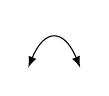
\begin{tikzpicture}
\draw[black, <->, >=latex] (-0.33, -0.5) .. controls (-0.125, 0) and (0.125, 0) .. (0.33, -0.5);
\end{tikzpicture}}

\newcommand{\CVdownInc}{%
\begin{tikzpicture}
\draw[black, ->, >=latex] (-0.5, -0.5) .. controls (-0.5, -0.3) and (-0.5, -0.1) .. (0,0);
\end{tikzpicture}}

\newcommand{\CVdownDec}{%
\begin{tikzpicture}[rotate=-90]
\draw[black, ->, >=latex] (-0.5, -0.5) .. controls (-0.5, -0.3) and (-0.5, -0.1) .. (0,0);
\end{tikzpicture}}

\begin{document}
	\noindent \hrulefill \\
	MATH-244 \semester \hfill Practice Problems Solutions\\
	Section 16.2 \hfill Pierre-Olivier Paris{\'e} \\\vspace*{-1cm}
	
	\noindent\hrulefill
	
	\spc	

	\exo{2}
	We have $x'(t) = 3t^2$ and $y'(t) = 4t^3$. So, the line integral becomes
		\begin{align*}
		\int_C (x/y) \, ds = \int_1^2 (t^3/t^4) \sqrt{9t^4 + 16 t^6} \, dt = 3 \int_1^2 t \sqrt{1 + (4t/3)^2} \, dt .
		\end{align*}
	By letting $u = 1 + (4t/3)^2$, we get 
		\begin{align*}
		\int_C (x/y) \, ds = \frac{1}{48} (73 \sqrt{73} - 125) \approx 10.390 .
		\end{align*}
		
	\spc
	
	\exo{8}
	We parametrize the circle $C_1$ described by $x^2 + y^2 = 2$ with $x = 2\cos (t)$ and $y = 2\sin (t)$. Since we only need the part of the circle going from $(2, 0)$ to $(0, 2)$, the parameter lies in $0 \leq t \leq \pi/2$ (a quarter of a circle). 
	
	We have $x'(t) = -2\sin (t)$ and $y'(t) = 2\cos (t)$. So, the contour integral is
		\begin{align*}
		\int_{C_1} x^2 dx + y^2 dy = \int_0^{\pi/2} (-8) \cos^2 (t) \sin (t) \, dt + 8 \int_0^{\pi/2} \sin^2 (t) \cos (t) \, dt = -8 \int_0^1 t^2 \, dt + 8 \int_0^1 t^2 \, dt .
		\end{align*}
	So we obtain
		\begin{align*}
		\int_{C_1} x^2 dx + y^2 dy = 0 .
		\end{align*}
		
	We parametrized the line segment $C_2$ by $x = 4t$ and $y = 2 + t$ where $0 \leq t \leq 1$. So $x'(t) = 4$ and $y'(t) = 1$. The contour integral is then
		\begin{align*}
		\int_{C_2} x^2 \, dx + y^2 \, dy = \int_0^1 64 t^2 \, dt + \int_0^1 (2 + t)^2 \, dt = \frac{64}{3} + \frac{8}{3} = 24 .
		\end{align*}
		
	If $C = C_1 \cup C_2$, then from the properties of the line integral, we obtain
		\begin{align*}
		\int_{C} x^2 dx + y^2 dy = \int_{C_1} x^2 dx + y^2 dy + \int_{C_2} x^2 \, dx + y^2 \, dy = 24 .
		\end{align*}				 

	\spc

	\exo{18}
	The expression in the line integral of a vector field $\vec{F}$ is $\vec{F} (\vec{r}(t)) \cdot \vec{r}'(t)$. This is also the following expression
		\begin{align*}
		\vec{F} (\vec{r}(t)) \cdot \vec{r}'(t) = \Vert \vec{F} \Vert \Vert \vec{r}' \Vert \cos (\theta (t) )
		\end{align*}
	where $\theta (t)$ is the angle between the two vectors. If $\theta (t)$ is always between $0$ and $\pi/2$, then the dot product is always positive because the cosine function is positive there and if $\theta (t)$ is always between $\pi/2$ and $\pi$, then the dot product is always negative because the cosine function is negative there.
	
	\begin{enumerate}
	\item[$C_1$.] The angle between the tangent vector $\vec{r}'(t)$ (which is always perpendicular to the radius of the circle) and the vector field is always between $0$ and $\pi/2$. So the dot product is always positive and so the integral is positive.
	\item[$C_2$.] Along most of the path, the angle between the tangent vector $\vec{r}'(t)$ (which is again perpendicular to the radius of the circle) and the vector field is between $\pi/2$ and $\pi$. The length of the vectors in the vector field are also bigger in this area of the curve. At the beginning of the curve $C_2$, we can see that the angle is less than $\pi/2$, but the modulus of the vectors in the vector field are small in this area. So this makes the dot product also small. So the all the weight goes on the part where the angles are between $\pi/2$ and $\pi$ and, thus, the line integral is negative.
	\end{enumerate}

	\spc
	
	\exo{22}
	We have $\vec{r}\,'(t) = (-\sin t) \vec{i} + \cos (t) \vec{j} + \vec{k}$. So,
		\begin{align*}
		\vec{F} (\vec{r}(t)) \cdot \vec{r}\,' = -\cos t \sin t  + \cos t \sin t + \cos t \sin t = \cos t \sin t .
		\end{align*}
	Thus, we obtain
		\begin{align*}
		\int_C \vec{F} \cdot d \vec{r} = \int_0^\pi \cos t \sin t \, dt = \int_0^\pi (1/2) \sin (2t) \, dt = 0.
		\end{align*}
		
	\spc
	
	\exo{41}
	The line segment is parametrize by
		\begin{align*}
		\vec{r} (t) = \left\langle 2t , t , 1 - t \right\rangle \quad (0 \leq t \leq 1 ) .
		\end{align*}
	The work done by the vector field over the line segment is given by the line integral of the vector field over the line segment. We have $\vec{r}\,' (t) = \left\langle 2 , 1 , -1 \right\rangle$ and
		\begin{align*}
		\vec{F} (\vec{r}(t)) = \left\langle 2t - t^2 , t - (1 - t)^2 , 1 - t - 4t^2 \right\rangle .
		\end{align*}
	So, the expression of the line integral is
		\begin{align*}
		W &= \int_0^1 \left\langle 2t - t^2 , t - (1 - t)^2 , 1 - t - 4t^2 \right\rangle \cdot \left\langle 2 , 1 , -1 \right\rangle \, dt \\
		&= \int_0^1 4t - 2t^2 + t - (1-t)^2 - 1 + t + 4t^2 \, dt \\
		&= 7/3
		\end{align*}


\end{document}